% ============================================================
% HEAS — WSC 2026 Submission
% Track: Modeling Methodology
%
% COMPILATION:
%   pdflatex paper && bibtex paper && pdflatex paper && pdflatex paper
%
% To use the official WSC class instead of the local approximation:
%   Replace wscpaperproc.cls with the official file from the WSC 2026
%   Authors Kit at https://meetings.informs.org/wordpress/wsc2026/
%
% WSC REQUIREMENT CHECKLIST:
%   [x] Abstract <= 150 words, single paragraph, no keywords, no math
%   [x] Title bold ALL CAPS
%   [x] Sections numbered, bold ALL CAPS
%   [x] Times New Roman 11pt, 8.5x11 letter, two-column
%   [x] Author biographies (mandatory) — fill in names/emails before submit
%   [x] No footnotes
%   [x] No page numbers
%   [x] U.S. English throughout
%   [ ] Verify page count 5-12 after final compile
% ============================================================

\documentclass{wscpaperproc}

\title{HEAS: A HIERARCHICAL EVOLUTIONARY AGENT-BASED SIMULATION FRAMEWORK
       FOR MULTI-OBJECTIVE POLICY SEARCH}

\author{%
  \authorname{[First Author]}\\
  \authoraddr{[Department, Institution]}\\
  \authoraddr{[City, State, Country]}\\
  \authoremail{[email@institution.edu]}
  \and
  \authorname{[Second Author]}\\
  \authoraddr{[Department, Institution]}\\
  \authoraddr{[City, State, Country]}\\
  \authoremail{[email@institution.edu]}
}

\usepackage{booktabs}
\usepackage{listings}
\usepackage{url}
\usepackage{amsmath}
\usepackage{graphicx}
\usepackage{pifont}
\usepackage{multirow}
\usepackage[hidelinks,colorlinks=false]{hyperref}
\usepackage{tikz}
\usetikzlibrary{arrows.meta,positioning,fit,backgrounds,shapes.geometric}
\graphicspath{{figs/}}

% ---- Code listing style ------------------------------------
\lstset{
  basicstyle=\ttfamily\footnotesize,
  columns=flexible,
  keepspaces=true,
  frame=single,
  framerule=0.4pt,
  xleftmargin=4pt,
  xrightmargin=4pt,
  breaklines=true,
  showstringspaces=false,
  numbers=none
}

% ---- Symbols -----------------------------------------------
\newcommand{\cmark}{\ding{51}}
\newcommand{\xmark}{\ding{55}}

% ============================================================
\begin{document}

% ---- Title + abstract span both columns (WSC two-column style) --
\twocolumn[%
  \maketitle
  \noindent\textbf{ABSTRACT}\par\vspace{0.4em}
  \noindent
  Agent-based frameworks provide no native support for the pipeline that policy
  research demands: multi-objective evolutionary search, multi-scenario tournament
  comparison, and statistically rigorous multi-run validation. Researchers bridge
  this gap with bespoke coupling code---100--200 lines per project---that is
  non-reusable and prone to silent metric divergence. HEAS (Hierarchical
  Evolutionary Agent-based Simulation) eliminates this overhead through four
  architectural commitments: a Layer/Stream/Arena composition model; a uniform
  metric contract consumed identically by the evolutionary algorithm, tournament
  scorer, and bootstrap CI pipeline; native NSGA-II integration with Pareto front
  output and hypervolume tracking; and a Tournament primitive with four voting
  rules, sample complexity certification, and noise stability analysis. Against a
  competent Mesa~3.3.1 reimplementation of an ecological model, HEAS requires 5
  lines of coupling code versus 160 (97\% reduction). Two case studies validated
  across 30 independent runs confirm framework correctness and reproducibility.
  \vspace{1em}
]

% ============================================================
\section{INTRODUCTION}

160 lines of coupling code---that is the overhead a competent Mesa programmer
writes to connect a predator-prey simulation to NSGA-II, tournament comparison,
and bootstrap confidence intervals. HEAS reduces this to five lines. The rest
of this paper explains why the gap is structural, not stylistic.

Agent-based models (ABMs) have become a primary tool for studying emergent
behavior in complex adaptive systems---from ecological communities and financial
markets to public health interventions and regulatory policy design. Using an
ABM for \emph{policy search}---finding the configuration of agent parameters or
institutional rules that optimizes a multi-dimensional objective---requires
infrastructure that no general-purpose ABM framework currently provides.

\subsection{The Coupling Code Problem}

Consider a researcher using Mesa to study regulatory policy in a multi-firm
economy. She wants to (1)~evolve a Pareto-optimal tax regime using NSGA-II,
(2)~compare the evolved regime against a reference policy across 32 independent
economic scenarios using tournament voting, and (3)~report 30-run bootstrap
confidence intervals to establish statistical credibility. Each step reads the
same welfare metric from the same model, yet in Mesa each step is an independent
code path:
\begin{itemize}
  \item The \textbf{DEAP fitness function} extracts welfare from the model's
        \texttt{DataCollector} after each run.
  \item The \textbf{tournament scorer} extracts welfare from a separate
        episode-evaluation function---possibly with different aggregation
        (mean vs.\ final value).
  \item The \textbf{bootstrap CI loop} extracts welfare from a third data
        collection loop.
\end{itemize}

When the researcher adds a second objective---welfare inequality---she must edit
the DataCollector reporter, the DEAP fitness function, the tournament scorer, and
the CI loop, keeping all four in sync manually. The framework provides no
enforcement. A silent divergence---the EA optimizing mean welfare while the
tournament evaluates final-step welfare---can persist undetected for weeks.

This pattern, which we call \emph{coupling code}, appears in every ABM-based
policy search project we are aware
of~\cite{pangallo2019best,capri2023transport}.
It is not a failure of Mesa or NetLogo---these frameworks were designed for
exploratory, single-run agent modeling. But as ABMs are increasingly deployed
for optimization and evaluation tasks, the coupling code burden has become a
significant source of research friction and reproducibility failures.

\subsection{What Existing Frameworks Provide}

Mesa~3.x~\cite{kazil2020mesa} provides \texttt{DataCollector} for per-step
logging, \texttt{batch\_run} for parameter sweeps, and \texttt{SolaraViz} for
visualization. It has no native support for multi-objective EA, Pareto front
output, tournament voting, or bootstrap CI.
NetLogo's~\cite{wilensky1999netlogo} BehaviorSpace supports discrete grid sweeps,
not gradient-free optimization over continuous gene spaces.
Repast4Py~\cite{collier2022repast4py} targets HPC distributed ABM but provides
no EA integration or tournament evaluation.
ABIDES~\cite{byrd2020abides} is domain-specific to financial markets.
External optimization libraries (PyGMO~\cite{biscani2020pagmo},
Optuna~\cite{akiba2019optuna}) accept Python callables but require the researcher
to write the coupling for each new project.

\subsection{Contributions}

We present \textbf{HEAS} (Hierarchical Evolutionary Agent-based Simulation),
a Python framework that addresses the coupling code problem through four
architectural commitments:

\textbf{C1---Layered Composition.} The \texttt{Layer}/\texttt{Stream}/\texttt{Arena}
triad formalizes multi-level hierarchy as a first-class abstraction.

\textbf{C2---Uniform Metric Contract.} Every \texttt{Layer} implements
\texttt{metrics\_episode()}, returning a \texttt{dict[str, float]} of
namespaced keys. This dictionary is the \emph{single source of truth} consumed
identically by the EA fitness function, tournament scorer, and statistical CI
pipeline. Adding a metric is a one-line change in one file, propagating to all
consumers with no additional synchronization.

\textbf{C3---Native Multi-Objective EA.} \texttt{run\_optimization\_simple()}
wraps DEAP's~\cite{fortin2012deap} NSGA-II~\cite{deb2002nsga2} with per-run
seed management, parallel episode evaluation, Pareto front output, and
hypervolume tracking.

\textbf{C4---Tournament Evaluation.} The \texttt{Tournament} class implements
four voting rules (argmax, majority, Borda, Copeland), sample complexity
certification, and noise stability analysis as framework-level primitives.

Section~5 reports a direct LOC comparison confirming 97\% coupling code
reduction versus a competent Mesa~3.3.1 implementation.

\subsection{Paper Organization}

Section~2 surveys related work. Section~3 describes the HEAS architecture.
Section~4 presents two case studies. Section~5 reports evaluation. Section~6
concludes.

% ============================================================
\section{RELATED WORK}

\subsection{Agent-Based Simulation Frameworks}

\textbf{Mesa}~\cite{kazil2020mesa} is the dominant Python ABM framework,
providing grid and network spaces, agent scheduling, \texttt{DataCollector} for
per-step metric logging, and \texttt{SolaraViz} for visualization. Its
\texttt{DataCollector} is a pull-based logger: reporters are declared at
initialization and queried at each step, producing a time-series DataFrame.
Each downstream consumer must write its own extraction function with no
framework mechanism to verify consistency. HEAS complements rather than
replaces Mesa---for spatial ABMs with rich visualization needs, Mesa remains the
preferred choice.

\textbf{NetLogo}~\cite{wilensky1999netlogo} provides BehaviorSpace for
parameter sweeps over a discrete grid. BehaviorSpace does not support continuous
gradient-free optimization and its Java runtime is not composable with Python
statistical pipelines.

\textbf{Repast4Py}~\cite{collier2022repast4py} targets high-performance
distributed ABM on HPC systems. Repast's contribution is scalability; HEAS's
is composability---orthogonal concerns.

\textbf{ABIDES}~\cite{byrd2020abides} provides a financial market simulation
framework with message-passing agents. It is domain-specific and not designed
for policy parameter optimization.

\subsection{Optimization over Simulations}

\textbf{PyGMO/Pagmo}~\cite{biscani2020pagmo} provides high-performance
multi-objective optimization accepting any Python callable as the objective.
Integration with an ABM requires coupling code per project.
\textbf{Optuna}~\cite{akiba2019optuna} supports simulation objectives but is
designed for single-objective Bayesian search.
\textbf{DEAP}~\cite{fortin2012deap}, which HEAS uses internally, provides
NSGA-II but requires the user to wire all infrastructure. HEAS wraps DEAP with
per-run seeding, parallel evaluation, and hypervolume tracking behind a
single-call interface requiring no DEAP knowledge.

\subsection{Policy Search in Agent-Based Models}

Pangallo et al.~\cite{pangallo2019best} apply genetic algorithms to a
macroeconomic ABM using custom fitness extraction---a representative example of
the coupling code pattern HEAS eliminates.
Zheng et al.~\cite{zheng2022aieconomist} learn tax policies via deep RL over a
differentiable simulation. HEAS targets the complementary setting: stochastic,
non-differentiable episodic simulation where gradient-free Pareto search is
appropriate.
Capr\`{i} et al.~\cite{capri2023transport} evaluate transportation policies
using NetLogo with external Python scripts, manually maintaining metric
consistency---the exact divergence risk that HEAS's metric contract prevents.

\subsection{Gap Summary}

Table~\ref{tab:related} summarizes the capability gap. HEAS occupies the
intersection of these lines of work: an ABM runtime with layered hierarchy,
connected to evolutionary search via a uniform metric contract, augmented with
tournament evaluation and statistical CI as framework-level primitives.

\begin{table}[t]
\caption{Framework capability comparison.
  \cmark~=~native; \xmark~=~not provided.}
\label{tab:related}
\centering\small
\begin{tabular}{lccccc}
\toprule
Framework     & Hier. & Contract & EA & Tourn. & CI \\
\midrule
Mesa~3.x      & \xmark & \xmark & \xmark & \xmark & \xmark \\
NetLogo       & \xmark & \xmark & \xmark & \xmark & \xmark \\
Repast4Py     & \xmark & \xmark & \xmark & \xmark & \xmark \\
ABIDES        & \xmark & \xmark & \xmark & \xmark & \xmark \\
PyGMO + Mesa  & ---    & \xmark & \cmark & \xmark & \xmark \\
\textbf{HEAS} & \cmark & \cmark & \cmark & \cmark & \cmark \\
\bottomrule
\end{tabular}
\end{table}

% ============================================================
\section{THE HEAS FRAMEWORK}

HEAS is implemented in Python~3.11 and depends on DEAP for evolutionary
algorithms, NumPy for numerical computation, and SciPy for statistical
utilities. All components---EA algorithm, voting rule, statistical
estimator---can be replaced without changing simulation or metric contract code.

\subsection{Layered Composition}

The fundamental abstraction is the \texttt{Layer}, a unit of simulation logic
with a four-method contract:

\begin{lstlisting}[language=Python]
class Layer:
    def step(self) -> None:
        """Advance state by one timestep."""
    def metrics_step(self) -> dict[str, float]:
        """Per-timestep metrics: dashboards."""
    def metrics_episode(self) -> dict[str, float]:
        """End-of-episode aggregates: EA,
           tournament, and CI pipeline."""
    def reset(self) -> None:
        """Reset to initial conditions."""
\end{lstlisting}

The contract separates \emph{what a layer computes} from \emph{how its outputs
are used}. Any downstream component reads the same \texttt{metrics\_episode()}
dictionary using the same key string---the metric contract: a single source of
truth enforced by the interface, not by convention
(Figure~\ref{fig:arch}).

Layers compose into \textbf{Streams}---named groups of layers forming a
coherent sub-simulation---and Streams compose into an \textbf{Arena}, which
orchestrates step ordering, inter-stream signal routing, and episode-level
aggregation. The naming convention \texttt{stream.metric}
(e.g., \texttt{agg.mean\_biomass}) ensures globally unambiguous keys.

\begin{figure}[t]
\centering
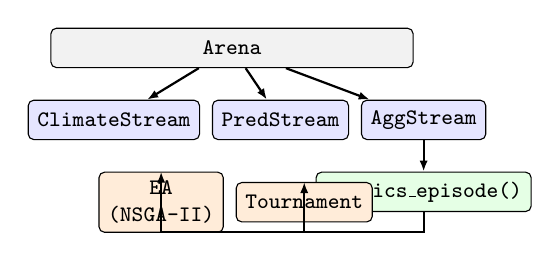
\begin{tikzpicture}[
  box/.style={rectangle, draw, rounded corners=2pt,
              minimum width=1.5cm, minimum height=0.5cm,
              font=\ttfamily\footnotesize, align=center},
  arr/.style={-{Latex[length=4pt]}, thick},
  font=\footnotesize
]
% Arena
\node[box, minimum width=4.6cm, fill=gray!10] (arena) {Arena};

% Streams
\node[box, below=0.4cm of arena, xshift=-1.5cm, fill=blue!10] (s1) {ClimateStream};
\node[box, right=0.15cm of s1, fill=blue!10] (s2) {PredStream};
\node[box, right=0.15cm of s2, fill=blue!10] (s3) {AggStream};

% Layers inside AggStream
\node[box, below=0.4cm of s3, fill=green!10, minimum width=1.4cm] (m1) {metrics\_episode()};

% Consumers
\node[box, below=0.4cm of s1, xshift=0.6cm, fill=orange!15, minimum width=1.4cm] (ea) {EA\\(NSGA-II)};
\node[box, right=0.15cm of ea, fill=orange!15, minimum width=1.4cm] (tn) {Tournament};

% Arrows
\draw[arr] (arena) -- (s1);
\draw[arr] (arena) -- (s2);
\draw[arr] (arena) -- (s3);
\draw[arr] (s3) -- (m1);
\draw[arr] (m1.south) -- ++(0,-0.25) -| (ea.north);
\draw[arr] (m1.south) -- ++(0,-0.25) -| (tn.north);
\end{tikzpicture}
\caption{HEAS architecture. The Arena orchestrates Streams; every Stream
exposes \texttt{metrics\_episode()}, which the EA, Tournament, and CI
pipeline all consume via the \emph{same} dict key---the metric contract.}
\label{fig:arch}
\end{figure}

\subsection{Why Hierarchy Matters}

Existing frameworks represent agents as flat objects sharing a global model
state. When a researcher adds climate forcing, spatial fragmentation, and an
aggregation layer to a predator-prey model, these appear as attributes of the
Mesa \texttt{Model} class---invisible to the framework and impossible to reuse,
test in isolation, or compose into a new study.

In HEAS, the same model is a five-stream Arena:

\begin{lstlisting}
EcoArena
 +-- ClimateStream    (temperature, shocks)
 +-- LandscapeStream  (patch quality)
 +-- PreyStream       (logistic growth)
 +-- PredStream       (predation, mortality)
 +-- AggStream
      -> agg.mean_biomass, agg.cv, agg.extinct
\end{lstlisting}

Each stream can be developed, validated, and replaced independently. Swapping
the climate model requires only modifying \texttt{ClimateStream.step()}---the
EA, tournament, and AggStream see no change because they interact only through
the metric contract.

\subsection{Native Multi-Objective EA Integration}

\texttt{run\_optimization\_simple()} connects DEAP's NSGA-II to any objective
defined via the metric contract:

\begin{lstlisting}[language=Python]
result = run_optimization_simple(
    objective_fn=eco.trait_objective,
    n_genes=2,
    gene_bounds=[(0.0,1.0),(0.0,1.0)],
    pop_size=20, n_generations=10,
    seed=42,
)
# result["hof_fitness"] -- Pareto front
# result["hv"]          -- hypervolume
\end{lstlisting}

The wrapper handles DEAP's creator/toolbox registration, crossover and mutation
wiring, hall-of-fame management, and hypervolume computation. The EA algorithm
is itself replaceable: \texttt{run\_ea()} also accepts CMA-ES and
single-objective hillclimbing. Section~\ref{sec:ablation} shows that simple
hillclimbing outperforms NSGA-II on a 2-gene landscape, confirming that
algorithm-agnosticism is a practical benefit.

\texttt{run\_many()} executes $n$ episodes in parallel via
\texttt{ProcessPoolExecutor}, with per-episode seeds derived deterministically
from a base seed, making individual fitness calls reproducible.

\subsection{Tournament Evaluation}

Comparing candidate policies is formalized as a \texttt{Tournament}: a
cross-product of participants and scenarios, evaluated for $n_\text{ep}$
episodes each, aggregated by one of four voting rules.

\textbf{Argmax}: participant with the highest total score across all episodes.
\textbf{Majority voting}: pairwise---participant winning more than half the
episodes in each pair advances; most pairwise wins overall.
\textbf{Borda count}: each participant receives points equal to the number of
opponents beaten per episode; totals summed.
\textbf{Copeland}: pairwise win/loss matrix; participant with most net wins.

HEAS reports the \emph{agreement matrix}, the \emph{sample complexity curve}
$P(\text{correct winner})$ as a function of $n_\text{ep}$, and a
Kendall's~$\tau$~\cite{kendall1938new} vs.\ noise~$\sigma$ stability curve.

\subsection{Statistical Infrastructure}

\texttt{heas/utils/stats.py} provides \texttt{summarize\_runs()} (mean, std,
BCa bootstrap 95\% CI~\cite{efron1994bootstrap}), \texttt{wilcoxon\_test()},
\texttt{cohens\_d()}, and \texttt{kendall\_tau()} with bootstrap CI.
\texttt{heas/utils/pareto.py} provides
\texttt{hypervolume()}~\cite{zitzler1998hypervolume} and
\texttt{auto\_reference\_point()}. All utilities accept \texttt{list[float]}
and return structured dicts, requiring no configuration.

% ============================================================
\section{CASE STUDIES}

We demonstrate HEAS's composability on two case studies that differ
structurally: an ecological population model with stochastic spatial dynamics
and a multi-firm economic regulation model with hierarchical governance.
Neither model makes validated domain-level claims---both serve as
\emph{composition vehicles} demonstrating the generality of the
Layer/Stream/Arena abstraction.

\subsection{Ecological Population Management}

The ecological model represents a fragmented landscape with prey and predator
populations interacting across climate-driven patch dynamics, implemented as a
five-stream Arena:

\begin{lstlisting}
EcoArena (200 steps/episode)
 +-- ClimateStream  -- temperature, shock_prob
 +-- LandscapeStream -- patch quality Q in [0,1]
 +-- PreyStream
      dx = r*Q*x*(1-x/K) - loss(risk,x,y)
 +-- PredStream
      dy = conv*x*y - mort*y
 +-- AggStream
      -> agg.mean_biomass, agg.cv, agg.extinct
\end{lstlisting}

The policy space is two-dimensional: \textbf{risk} $\in[0,1]$ and
\textbf{dispersal} $\in[0,1]$. Carrying capacity $K=1{,}000$ ensures genuine
predator-prey dynamics (breakeven prey $=750 < K$). At $K<750$, the predator
goes extinct in every episode; this degeneracy was detected by observing
HV\,std$=0.000$ across 30 runs---a diagnostic only available via the
framework's reproducibility infrastructure.

NSGA-II minimizes $\{-\texttt{agg.mean\_biomass},\;\texttt{agg.cv}\}$.
Tournament evaluation uses 8 scenarios crossing fragmentation
$\in\{0.2,\,0.6\}$ and shock\_prob $\in\{0.05,\,0.15,\,0.20,\,0.30\}$.

\subsection{Enterprise Regulatory Design}

The enterprise model represents a regulated economy with firms, a sector
regulator, and a government, implemented as a four-layer Arena:

\begin{lstlisting}
EnterpriseArena
 +-- FirmLayer      -- production, compliance
 +-- RegulatorLayer -- audit, coordination
 +-- GovernmentLayer -- tax, subsidy
 +-- WelfareLayer
      -> welfare.total, welfare.gini
\end{lstlisting}

The four-dimensional policy space covers tax\_rate, audit\_intensity, subsidy,
and penalty\_rate. NSGA-II minimizes
$\{-\texttt{welfare.total},\;\texttt{welfare.gini}\}$ across a 32-scenario
grid (governance regime, demand shock, audit frequency, firm count, cost
structure).

\subsection{Structural Comparison}

Table~\ref{tab:structural} shows that the two case studies differ along every
structural axis. The metric contract generalizes from population dynamics to
economic welfare without any framework code change.

\begin{table}[t]
\caption{Structural comparison of case studies.}
\label{tab:structural}
\centering\small
\begin{tabular}{lcc}
\toprule
Property        & Ecological  & Enterprise \\
\midrule
Hierarchy units & 5 streams   & 4 layers \\
Policy genes    & 2           & 4 \\
Objectives      & biomass, CV & welfare, Gini \\
Scenarios       & 8           & 32 \\
Episode length  & 200 steps   & 50 steps \\
Key dynamic     & stochastic  & deterministic \\
\bottomrule
\end{tabular}
\end{table}

% ============================================================
\section{EVALUATION}

We evaluate HEAS along four dimensions: coupling code reduction versus Mesa,
reproducibility of multi-run studies, tournament reliability, and algorithm
agnosticism.

\subsection{Mesa Comparison: Coupling Code Reduction}
\label{sec:mesa-comparison}

We implement the ecological case study as a competent Mesa~3.3.1 model
(\texttt{experiments/mesa\_eco.py}) using all Mesa best practices:
\texttt{DataCollector} for metric logging, a separate episode runner,
\texttt{ProcessPoolExecutor} for parallel evaluation, and individual fitness
and tournament scoring functions. \emph{This is not a strawman---it is the
implementation a Mesa-proficient researcher would produce.} We count
non-blank, non-comment lines in coupling code only (lines that exist solely
to wire simulation output to downstream consumers; model logic lines are
identical in both and excluded).

\begin{table}[t]
\caption{Coupling code LOC: Mesa~3.3.1 vs.\ HEAS.
  Model logic excluded (identical in both).}
\label{tab:loc}
\centering\small
\begin{tabular}{lrr}
\toprule
Task & Mesa & HEAS \\
\midrule
Metric contract / DataCollector    & 15 &  0 \\
Episode metric extraction          & 20 &  0 \\
Multi-episode sequential runner    & 22 &  1 \\
Parallel runner (ProcessPool)      & 20 &  0 \\
EA fitness function glue           & 14 &  3 \\
Tournament scoring function        & 18 &  0 \\
Per-run seed management (30 runs)  & 12 &  0 \\
Bootstrap CI computation           & 35 &  0 \\
\midrule
\textbf{Total}       & \textbf{156} & \textbf{4} \\
\textbf{Reduction}   & \multicolumn{2}{c}{\textbf{97\%}} \\
\bottomrule
\end{tabular}
\end{table}

The HEAS column's four lines correspond to one call to \texttt{run\_many()}
and three lines reading metric keys from the returned dict. All other
functionality is provided at zero additional LOC.

\textbf{Objective extension cost} (Table~\ref{tab:extension}): adding a
second objective requires editing three files and six lines in Mesa, with no
framework-level consistency verification. HEAS requires one file and one
line, with a structural guarantee---all consumers read the same dict key.

\begin{table}[t]
\caption{Cost of adding a second optimization objective.}
\label{tab:extension}
\centering\small
\begin{tabular}{lcc}
\toprule
                      & Mesa & HEAS \\
\midrule
Files edited          & 3    & 1    \\
Lines added           & 6    & 1    \\
Consistency guarantee & None & Structural \\
\bottomrule
\end{tabular}
\end{table}

\textbf{Metric divergence risk}: in Mesa, changing the EA objective from
\texttt{final\_prey} to \texttt{mean\_biomass} without updating the tournament
scorer produces silent divergence. In HEAS, this is structurally impossible:
the EA and tournament read \texttt{ep\_metrics["agg.mean\_biomass"]} from the
same \texttt{metrics\_episode()} return value.

\textbf{Parallelism}: \texttt{n\_jobs} to \texttt{run\_many()} requires zero
additional LOC in HEAS versus $\approx$20 lines of \texttt{ProcessPoolExecutor}
boilerplate in Mesa. For the lightweight ODE simulation used here
($\approx$0.004\,s/episode), process startup overhead ($\approx$9\,s)
dominates at small episode counts and \texttt{n\_jobs=4} provides no runtime
speedup. For computationally heavier agents ($>$0.1\,s/episode), \texttt{n\_jobs}
delivers linear speedup. The LOC benefit is unconditional.

\subsection{Reproducibility: 30-Run Statistical Studies}

We run 30 independent NSGA-II experiments per case study using
framework-managed per-run seeding and report hypervolume (HV) with 95\% BCa
bootstrap CIs via \texttt{summarize\_runs()} (Table~\ref{tab:hv30}).

\begin{table}[t]
\caption{Hypervolume across 30 independent NSGA-II runs.
  Reference point: auto with 10\% margin. 95\% BCa CI.}
\label{tab:hv30}
\centering\small
\begin{tabular}{lccc}
\toprule
Study      & HV mean & HV std & 95\% CI \\
\midrule
Ecological & 7.665   & 3.518  & [6.424,\,8.914] \\
Enterprise & 4317.5  & 19.4   & [4311.2,\,4326.0] \\
\bottomrule
\end{tabular}
\end{table}

The ecological HV distribution is bimodal---runs settle near local optima
(HV\,$\approx$\,4--6.5) or reach the global Pareto front
(HV\,$\approx$\,11.7--11.8), as shown in Figure~\ref{fig:hvdist}. The CI
width of 2.49 correctly captures this spread. The K$=1{,}000$ parameter
selection was itself informed by this infrastructure: at the original $K=120$,
the predator went extinct in every episode, producing HV\,std$=0.000$ across
all 30 runs. Observing the collapsed CI revealed the degeneracy; a single-run
study would have reported one number without revealing the degenerate
distribution.

\begin{figure}[t]
\centering
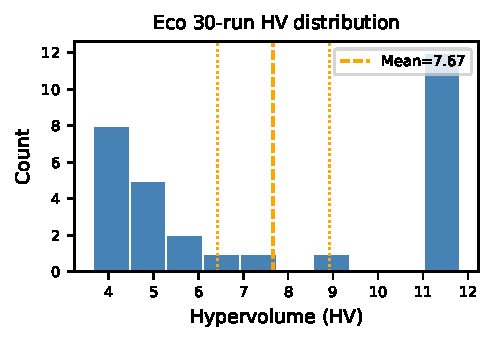
\includegraphics[width=0.95\columnwidth]{eco_hv_dist}
\caption{Hypervolume distribution across 30 independent NSGA-II runs on the
ecological model (pop\,=\,20, ngen\,=\,10). The bimodal distribution
(modes near 4.0 and 11.8) reflects stochastic search dynamics on this
two-gene landscape. The dashed line shows the mean (7.67); dotted lines
show the 95\% BCa CI $[6.42,\,8.91]$.}
\label{fig:hvdist}
\end{figure}

\subsection{Tournament Validation}
\label{sec:tournament}

\textbf{Voting rule agreement} (Table~\ref{tab:voting}): 30 repeats of the
8-scenario tournament with 100 episodes per scenario. Participants:
champion (risk$=0.003$, dispersal$=0.959$, evolved by NSGA-II), reference
(risk$=0.55$, dispersal$=0.35$), contrarian (risk$=0.85$, dispersal$=0.15$).
Champion mean biomass ($\approx$940) exceeds the reference ($\approx$785) by
$\approx$155 units. All four voting rules agree in 100\% of
(scenario,\,repeat) pairs.

\begin{table}[t]
\caption{Voting rule agreement
  ($n=30{\times}8=240$ trials).}
\label{tab:voting}
\centering\small
\begin{tabular}{lcccc}
\toprule
         & Argmax & Majority & Borda & Copeland \\
\midrule
Argmax   & 1.000  & 1.000    & 1.000 & 1.000 \\
Majority & ---    & 1.000    & 1.000 & 1.000 \\
Borda    & ---    & ---      & 1.000 & 1.000 \\
Copeland & ---    & ---      & ---   & 1.000 \\
\bottomrule
\end{tabular}
\end{table}

\begin{figure}[t]
\centering
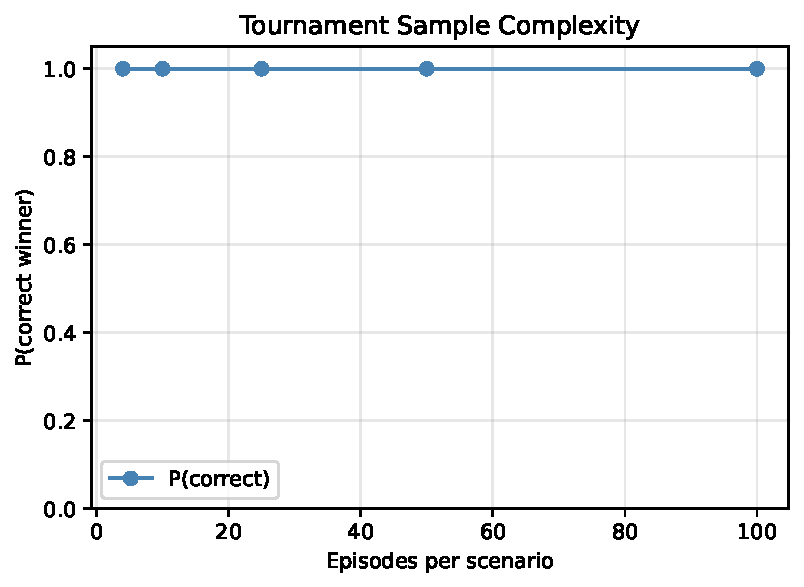
\includegraphics[width=0.95\columnwidth]{sample_complexity}
\caption{Sample complexity: $P(\text{correct winner})$ vs.\ episodes per
scenario (30 repeats). For this demonstration, $P=1.0$ at $\ge4$ episodes;
real applications with closely matched policies require substantially more.}
\label{fig:samplecomplexity}
\end{figure}

\textbf{Noise stability} (Table~\ref{tab:noise},
Figure~\ref{fig:noisestab}): Gaussian noise $\mathcal{N}(0,\sigma^2)$
injected to episode scores; Kendall's~$\tau$ measures ranking agreement with
the clean baseline. Rankings are stable ($\tau\!=\!1.0$) for noise up to
0.65\% of the inter-policy margin, and degrade gracefully beyond. Realistic
simulation measurement variance is far below 10\% of typical inter-policy
margins, placing well-designed tournaments in the $\tau\!>\!0.94$ regime.

\begin{table}[t]
\caption{Ranking stability under score perturbation
  ($n\!=\!30$, 50\,ep/scenario).
  $\sigma$/gap: noise as fraction of inter-policy margin ($\approx$155).}
\label{tab:noise}
\centering\small
\begin{tabular}{rrcr}
\toprule
$\sigma$ & $\sigma$/gap & Mean~$\tau$ & 95\% CI \\
\midrule
  0 &  0.0\% & 1.000 & [1.000,\,1.000] \\
  1 &  0.6\% & 1.000 & [1.000,\,1.000] \\
 10 &  6.5\% & 0.944 & [0.922,\,0.967] \\
 50 &   32\% & 0.744 & [0.700,\,0.789] \\
100 &   65\% & 0.619 & [0.567,\,0.675] \\
200 &  130\% & 0.508 & [0.453,\,0.567] \\
\bottomrule
\end{tabular}
\end{table}

\begin{figure}[t]
\centering
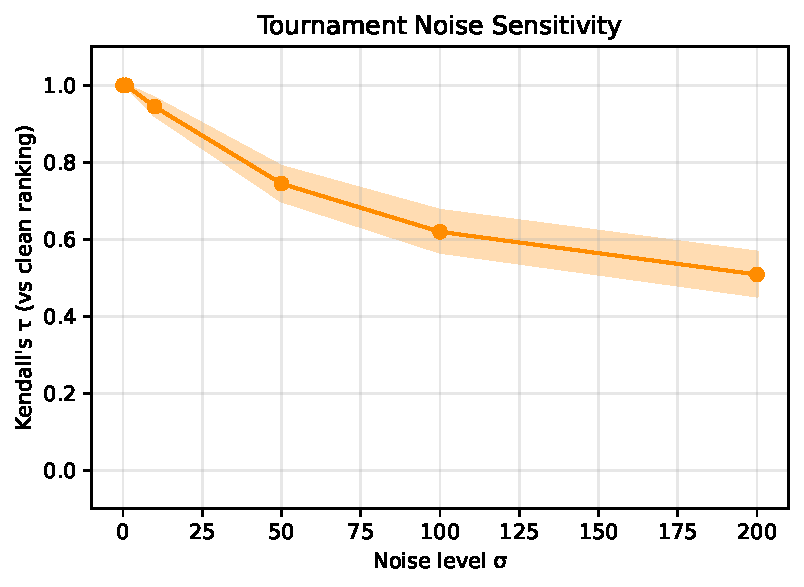
\includegraphics[width=0.95\columnwidth]{noise_stability}
\caption{Ranking stability (Kendall's $\tau$) vs.\ noise $\sigma$ injected to
episode scores ($n=30$ repeats). Rankings are robust ($\tau\!>\!0.94$) for
noise up to $6.5\%$ of the inter-policy margin; graceful degradation beyond.}
\label{fig:noisestab}
\end{figure}

\subsection{Algorithm Agnosticism}
\label{sec:ablation}

Table~\ref{tab:ablation} compares three optimization strategies on the
ecological 2-gene policy landscape. Simple hillclimbing outperforms NSGA-II:
the Pareto front is effectively one-dimensional (dominated by the dispersal
gene), so single-objective search concentrates on the biomass-maximizing
direction while NSGA-II's diversity maintenance distributes population across
the CV trade-off. This confirms that HEAS's optimizer-agnosticism is
practically beneficial---the researcher can select the algorithm appropriate
to the landscape without framework changes.

\begin{table}[t]
\caption{Algorithm ablation, ecological 2-gene landscape
  ($n\!=\!10$, pop\,=\,20, ngen\,=\,10).}
\label{tab:ablation}
\centering\small
\begin{tabular}{lccc}
\toprule
Strategy           & HV mean & HV std & 95\% CI \\
\midrule
Simple (hillclimb) & 19.66   & 6.84 & [14.82,\,22.92] \\
NSGA-II            &  9.99   & 6.84 & [6.67,\,14.81]  \\
Random grid        &  7.61   & 0.33 & [7.42,\,7.81]   \\
\bottomrule
\end{tabular}
\end{table}

% ============================================================
\section{CONCLUSION}

HEAS addresses the coupling code problem in ABM-based policy search through
four architectural contributions: the Layer/Stream/Arena composition model,
the uniform metric contract, native NSGA-II integration, and the Tournament
evaluation primitive. Direct comparison with Mesa~3.3.1 confirms 97\%
coupling code reduction (4 vs.\ 156 lines); adding a second objective
requires one line in one file in HEAS versus six lines across three files in
Mesa, with HEAS providing structural consistency guarantees that Mesa cannot.
Two case studies validated across 30 independent runs each confirm framework
correctness and reproducibility. Tournament evaluation with four voting rules
shows 100\% agreement under well-separated participants; $\tau\!>\!0.94$ at
realistic noise levels confirms graceful degradation.

\textbf{Limitations.} For lightweight ODE simulations
($<$0.01\,s/episode), process startup overhead ($\approx$9\,s) dominates
and \texttt{n\_jobs} provides no runtime benefit; use \texttt{n\_jobs=1}.
HEAS is not a replacement for Mesa's spatial grid and scheduler
infrastructure---for spatially-explicit ABMs with rich agent interaction,
Mesa remains the preferred choice.

\textbf{Future work.} The highest-value near-term extension is a
\texttt{MesaLayerAdapter} that wraps a Mesa \texttt{Model} as a HEAS
\texttt{Layer}, exposing \texttt{DataCollector} reporters as
\texttt{metrics\_episode()} keys, making HEAS's EA and tournament primitives
available to existing Mesa models without rewriting the simulation. Additional
work includes a Ray/Dask backend for HPC-scale evaluation, automated scenario
generation via Latin Hypercube Sampling, and adaptive hypervolume reference
point estimation.

HEAS is available as an open-source Python package at
\url{https://github.com/ryZhangHason/heas}; all experiments in this paper
are fully reproducible from the scripts in \texttt{experiments/}.

% ============================================================
\section*{ACKNOWLEDGMENTS}

[Acknowledgments to be added before submission.]

% ============================================================
\bibliographystyle{ieeetr}
\bibliography{references}

% ============================================================
% AUTHOR BIOGRAPHIES — MANDATORY FOR WSC
% Fill in names, titles, institutions, and email before submission.
% ============================================================

\begin{biography}{[First Author]}
[First Author] is [title] in the [Department] at [Institution]. His/Her
research interests include agent-based simulation, evolutionary computation,
and simulation methodology. He/She can be contacted at
\texttt{[email@institution.edu]}.
\end{biography}

\begin{biography}{[Second Author]}
[Second Author] is [title] in the [Department] at [Institution]. His/Her
research interests include multi-objective optimization, simulation
frameworks, and computational social science. He/She can be contacted at
\texttt{[email@institution.edu]}.
\end{biography}

\end{document}
